% This file was converted to LaTeX by Writer2LaTeX ver. 1.0.2
% see http://writer2latex.sourceforge.net for more info
\documentclass[twoside,letterpaper]{article}
\usepackage[latin1]{inputenc}
\usepackage[T1]{fontenc}
\usepackage[english]{babel}
\usepackage{amsmath}
\usepackage{amssymb,amsfonts,textcomp}
\usepackage{color}
\usepackage{array}
\usepackage{supertabular}
\usepackage{hhline}
\usepackage{hyperref}
\usepackage[all]{hypcap} 
\hypersetup{pdftex, colorlinks=true, linkcolor=blue, citecolor=blue, filecolor=blue, urlcolor=blue, pdftitle=SOFTWARE REQUIREMENTS SPECIFICATION (SRS) TEMPLATE, pdfauthor=Serta\c{c} Karahoda, pdfsubject=, pdfkeywords=}
\usepackage[pdftex]{graphicx}
\usepackage{tikz-uml}
% Outline numbering
\setcounter{secnumdepth}{5}
\renewcommand\thesection{\arabic{section}}
\renewcommand\thesubsection{\arabic{section}.\arabic{subsection}}
\renewcommand\thesubsubsection{\arabic{section}.\arabic{subsection}.\arabic{subsubsection}}
\renewcommand\theparagraph{\arabic{section}.\arabic{subsection}.\arabic{subsubsection}.\arabic{paragraph}}
\renewcommand\thesubparagraph{\arabic{section}.\arabic{subsection}.\arabic{subsubsection}.\arabic{paragraph}.\arabic{subparagraph}}
\makeatletter
\newcommand\arraybslash{\let\\\@arraycr}
\makeatother
% Page layout (geometry)
\setlength\voffset{-1in}
\setlength\hoffset{-1in}
\setlength\topmargin{0.5in}
\setlength\oddsidemargin{1in}
\setlength\evensidemargin{1in}
\setlength\textheight{8.278in}
\setlength\textwidth{6.5in}
\setlength\footskip{0.561in}
\setlength\headheight{0.5in}
\setlength\headsep{0.461in}
% Footnote rule
\setlength{\skip\footins}{0.0469in}
\renewcommand\footnoterule{\vspace*{-0.0071in}\setlength\leftskip{0pt}\setlength\rightskip{0pt plus 1fil}\noindent\textcolor{black}{\rule{0.25\columnwidth}{0.0071in}}\vspace*{0.0398in}}
% Pages styles
\makeatletter
\newcommand\ps@Standard{
  \renewcommand\@oddhead{\selectlanguage{english}\rmfamily\color{black} Sabanc{\i} University CS Department Instructional Use\hfill \hfill Scheduler}
  \renewcommand\@evenhead{\@oddhead}
  \renewcommand\@oddfoot{\foreignlanguage{english}{\textcolor{black}{\centerline{\thepage{}}}}}
  \renewcommand\@evenfoot{\@oddfoot}
  \renewcommand\thepage{\arabic{page}}
}
\newcommand\ps@Preface{
  \pagenumbering{Roman}
  \renewcommand\@oddhead{\selectlanguage{english}\rmfamily\color{black} Sabanc{\i} University CS Department Instructional Use\hfill \hfill Scheduler}
  \renewcommand\@evenhead{\@oddhead}
  \renewcommand\@oddfoot{\foreignlanguage{english}{\textcolor{black}{\centerline{\thepage{}}}}}
  \renewcommand\@evenfoot{\@oddfoot}
  \renewcommand\thepage{\roman{page}}
}
\newcommand\ps@Appendix{
  \renewcommand\@oddhead{}
  \renewcommand\@evenhead{\@oddhead}
  \renewcommand\@oddfoot{}
  \renewcommand\@evenfoot{\@oddfoot}
  \renewcommand\thepage{\arabic{page}}
}

\newcommand{\featuresection}[1] {
\subsubsection[System feature: #1]{\selectlanguage{english}\rmfamily\bfseries\color{black} System feature: #1}
}

\newcommand{\sequencediagramsection}[1] {
\subsubsection[Sequence diagram: #1]{\selectlanguage{english}\rmfamily\bfseries\color{black} Sequence diagram: #1}
}
\makeatother
\pagestyle{Standard}
\setlength\tabcolsep{1mm}
\renewcommand\arraystretch{1.3}
% footnotes configuration
\makeatletter
\renewcommand\thefootnote{\arabic{footnote}}
\makeatother
\title{SOFTWARE REQUIREMENTS SPECIFICATION (SRS)}
\author{Serta\c{c} Karahoda}
\date{16 March 2015}
\setlength\parindent{0pt}
\begin{document}
\setcounter{page}{1}\pagestyle{Preface}

\vspace*{1.5in}
{\centering\selectlanguage{english}\bfseries\color{black}
SOFTWARE REQUIREMENTS SPECIFICATION (SRS) FOR 
\par}

\bigskip

{\centering\selectlanguage{english}\bfseries\color{black}
SCHEDULER
\par}


\bigskip


\bigskip


\bigskip


\bigskip

{\centering\selectlanguage{english}\bfseries\color{black}
Version 1.0
\par}

{\centering\selectlanguage{english}\bfseries\color{black}
16 March 2015
\par}


\bigskip


\bigskip

{\centering\selectlanguage{english}\bfseries\color{black}
Prepared for:
\par}

{\centering\selectlanguage{english}\bfseries\color{black}
Ramin Armanfar <raminarmanfar@sabanciuniv.edu>

\par}


\bigskip


\bigskip

{\centering\selectlanguage{english}\bfseries\color{black}
Prepared by:
\par}

{\centering\selectlanguage{english}\bfseries\color{black}
Berk \c{C}iri\c{s}ci <berkcirisci@sabanciuniv.edu>

Elif Meri\c{c} <elifmeric@sabanciuniv.edu>

Pamir Mundt <pamirmundt@sabanciuniv.edu>

Serta\c{c} Karahoda <skarahoda@sabanciuniv.edu>

Yavuz Selim Emir <yavuzselim@sabanciuniv.edu>
\par}

\clearpage{\centering\selectlanguage{english}\bfseries\color{black}
SCHEDULER SRS
\par}


\bigskip

{\centering\selectlanguage{english}\bfseries\color{black}
PREFACE

\smallskip

RECORD OF CHANGES
\par}


\bigskip

\begin{flushleft}
\tablehead{}
\begin{supertabular}{|m{0.47685984in}|m{1.2418196in}|m{1.3587599in}|m{0.23375985in}|m{2.0462599in}|m{0.7337598in}|}
\hline
~

\centering \selectlanguage{english}\color{black} Change number &
~

\centering \selectlanguage{english}\color{black} Date completed &
~

\centering \selectlanguage{english}\color{black} Location of change
(e.g., page or figure \#) &
\centering \selectlanguage{english}\bfseries\color{black} A\newline
M\newline
D &
~

\centering \selectlanguage{english}\color{black} Brief description of
change &
~

\centering\arraybslash \selectlanguage{english}\color{black} Author\\\hline
\centering{0}
 &
\centering{15 March 2015}
 &
All
 &
\centering{A}
 &
 The document created
 &
 \vspace{0.05in}
 Serta\c{c}, Yavuz
 \\\hline
 \centering{1}
 &
\centering{22 March 2015}
 &
Section 2
 &
\centering{M}
 &
 User Requirements added
 &
 \vspace{0.05in}
 Pamir
 \\\hline
 \centering{2}
 &
\centering{22 March 2015}
 &
Section 4.2
 &
\centering{M}
 &
 System Requirements added
 &
 \vspace{0.05in}
 Serta\c{c}, Yavuz, Berk
 \\\hline
  \centering{3}
 &
\centering{28 March 2015}
 &
Section 3
 &
\centering{M}
 &
 System Architecture added
 &
 \vspace{0.05in}
 Serta\c{c}, Yavuz
 \\\hline
 \centering{4}
 &
\centering{28 March 2015}
 &
Section 2
 &
\centering{M}
 &
 Use case diagram added
 &
 \vspace{0.05in}
 Serta\c{c}, Yavuz
 \\\hline
  \centering{5}
 &
\centering{28 March 2015}
 &
Section 4
 &
\centering{M}
 &
 Sequence diagrams added
 &
 \vspace{0.05in}
 Serta\c{c}, Yavuz, Berk
 \\\hline
  \centering{6}
 &
\centering{29 March 2015}
 &
Section 5, 6, 7
 &
\centering{D}
 &
 Useless sections deleted
 &
 \vspace{0.05in}
 Serta\c{c}
 \\\hline
   \centering{7}
 &
\centering{29 March 2015}
 &
Section 1.4
 &
\centering{M}
 &
 Unexplained terms added
 &
 \vspace{0.05in}
 Serta\c{c}
 \\\hline
\centering{8}
 &
\centering{29 March 2015}
 &
Section 2.2
 &
\centering{M}
 &
 Related section, figure links added 
 &
 \vspace{0.05in}
 Berk
 \\\hline
 \centering{9}
 &
\centering{29 March 2015}
 &
Section 2.2
 &
\centering{M}
 &
 Some functions added 
 &
 \vspace{0.05in}
 Pamir
 \\\hline
  \centering{10}
 &
\centering{29 March 2015}
 &
Section 2.8
 &
\centering{A}
 &
 Mockups 
 &
 \vspace{0.05in}
 Serta\c{c}
 \\\hline
\end{supertabular}
\end{flushleft}
{\selectlanguage{english}\color{black}
\foreignlanguage{english}{*}\foreignlanguage{english}{\textbf{A}}\foreignlanguage{english}{
- ADDED
\ }\foreignlanguage{english}{\textbf{M}}\foreignlanguage{english}{ -
MODIFIED
\ }\foreignlanguage{english}{\textbf{D}}\foreignlanguage{english}{ -
DELETED}}

\clearpage{\centering\selectlanguage{english}\bfseries\color{black}
\foreignlanguage{english}{\MakeUppercase{\ }}\foreignlanguage{english}{\MakeUppercase{SCHEDULER SRS}}
\par}

{\centering\selectlanguage{english}\bfseries\color{black}
TABLE OF CONTENTS
\par}


\bigskip

{\selectlanguage{english}\bfseries\color{black}
Section\ \ Page}

\setcounter{tocdepth}{9}
\renewcommand\contentsname{}
\tableofcontents

\bigskip

\clearpage\clearpage\setcounter{page}{1}\pagestyle{Standard}
\section[INTRODUCTION]{\selectlanguage{english}\rmfamily\bfseries\color{black}
INTRODUCTION}

\subsection[IDENTIFICATION]{\selectlanguage{english}\rmfamily\bfseries\color{black}
IDENTIFICATION}

{\selectlanguage{english}\color{black}
\begin{flushleft}The software system being considered for development is referred to as course scheduler. \ The customer providing specifications
for the system is Ramin Armanfar. \ The ultimate
customer, or end-user, of the system will be students of Sabanc{\i}  University, especially undergraduate students. \ This is a new project effort, so the
version under development is version 1.0.\end{flushleft}}

\subsection[PURPOSE]{\selectlanguage{english}\rmfamily\bfseries\color{black}
PURPOSE}

{\selectlanguage{english}\color{black}
\begin{flushleft}The purpose of the system under development is to make course schedule for Sabanc\i{} University students. \ The main goal is to help students before and during the registration period. \ While the system will be used by Sabanc{\i} University students,
this document is intended to be read and understood by Teaching Assitants and Instructor of Software Engineering course.\end{flushleft}}

\subsection[SCOPE]{\selectlanguage{english}\rmfamily\bfseries\color{black}
SCOPE}

{\selectlanguage{english}\color{black}
\begin{flushleft}
This software system will be a course scheduling application for Sabanc\i{} University students. \ The application is based on a cross platform Java form application. \ The project will be developed in 4 months by 5 software engineers. \ There will be no sponsor or any investor. \ It has GPL license, it can be maintained and contributed by volunteer developers.

\end{flushleft}}

\subsection[GLOSSARY]{\selectlanguage{english}\rmfamily\bfseries\color{black}
GLOSSARY}
{\selectlanguage{english}\itshape\color{black}}

\begin{flushleft}
\tablehead{}
\begin{supertabular}{|m{1.3587599in}|m{5.00806in}|}
\hline
\centering \selectlanguage{english}\bfseries\color{black} Term or
Acronym &
\centering\arraybslash \selectlanguage{english}\bfseries\color{black}
Definition\\\hline
\selectlanguage{english}\color{black} \textbf{Alpha test} &
\selectlanguage{english}\color{black} Limited release(s) to selected,
outside testers\\\hline
\selectlanguage{english}\color{black} \textbf{Beta test} &
\selectlanguage{english}\color{black} Limited release(s) to cooperating
customers wanting early access to developing systems\\\hline
\selectlanguage{english}\color{black} \textbf{Final test} &
\selectlanguage{english}\color{black} aka, Acceptance test, release of
full functionality to customer for approval\\\hline
\selectlanguage{english}\color{black} \textbf{Bannerweb} &
\selectlanguage{english}\color{black} A course registration system for Sabanc{\i} University\\\hline
\selectlanguage{english}\color{black} \textbf{Cross platform }&
\selectlanguage{english}\color{black} Systems that can run on different operating system like Windows, Linux and Mac OS\\\hline
\selectlanguage{english}\color{black} \textbf{Java} &
\selectlanguage{english}\color{black} An object oriented, cross platform programming language \\\hline
\selectlanguage{english}\color{black} \textbf{GPL} &
\selectlanguage{english}\color{black} GNU General Public License is a free software license, which guarantees end users the freedoms to use, study, share, and modify the software. \\\hline
\selectlanguage{english}\color{black} \textbf{CRN} &
\selectlanguage{english}\color{black} Course Reference Number  \\\hline
\selectlanguage{english}\color{black} \textbf{Middleware} &
\selectlanguage{english}\color{black} The software that connects software components\\\hline
\selectlanguage{english}\color{black} \textbf{Parser} &
\selectlanguage{english}\color{black} a software component that takes input data and builds a data structure\\\hline
\selectlanguage{english}\color{black} \textbf{Boolean Type} &
\selectlanguage{english}\color{black} A data type that has only two value, true and false\\\hline

\end{supertabular}
\end{flushleft}

\clearpage

\subsection[OVERVIEW]{\selectlanguage{english}\rmfamily\bfseries\color{black}
OVERVIEW}

\begin{flushleft}{\selectlanguage{english}\color{black}
Section 2 of this document describes the system under development from a
holistic point of view. \ Functions, characteristics, constraints,
assumptions, dependencies, and overall requirements are defined from
the system-level perspective.}


\bigskip

{\selectlanguage{english}\color{black}
Section 3 of this document describes the architecture of the
system being developed. \ It shows relations between system components with high-level graphical representation.}


\bigskip

{\selectlanguage{english}\color{black}
Section 4 of this document describes the specific requirements of the
system being developed. \ Interfaces, features, and specific
requirements are enumerated and described to a degree sufficient for a
knowledgeable designer or coder to begin crafting an architectural
solution to the proposed system.}

\end{flushleft}

\clearpage\section[USER REQUIREMENTS DEFINITION]{\selectlanguage{english}\rmfamily\bfseries\color{black}
USER REQUIREMENTS DEFINITION}

\subsection[PRODUCT
PERSPECTIVE]{\selectlanguage{english}\rmfamily\bfseries\color{black}
PRODUCT PERSPECTIVE}

{\selectlanguage{english}\color{black}
Scheduler is a self-contained, standalone software that helps the Sabanc\i{} Univeristy students to efficiently create their own schudules without any external application. \ Although the application has a self-contained structure, it uses some webpages of Sabanc\i{} University as sources. \ It will be explained with details in section 2.5.}

\subsection[PRODUCT
FUNCTIONS]{\selectlanguage{english}\rmfamily\bfseries\color{black}
PRODUCT FUNCTIONS}

\subsubsection[Configuration of User Information
]{\selectlanguage{english}\rmfamily\bfseries\color{black}
Configuration of User Information}

{\selectlanguage{english}\color{black}
Scheduler shall open a configuration page as the user opens the Scheduler application for first time. The user shall fill the following sections in the configuration section:}

\begin{itemize}
			\item Major and minor program(s)
			\item Starting term for each programs
			\item Current term	
		\end{itemize}
	
\smallskip

{\selectlanguage{english}\color{black}
\emph{\textbf{Related system features:}} Section \ref{sssec:importCourse}, Section \ref{sssec:importRestrictions}, Section \ref{sssec:importDegree}}

\smallskip

{\selectlanguage{english}\color{black}
\emph{\textbf{Related sequence diagrams:}} Figure \ref{fig:ConfigureDiagram}, Figure \ref{fig:UpdateDiagram}}

\subsubsection[Degree Requirements
]{\selectlanguage{english}\rmfamily\bfseries\color{black}
	Degree Requirements}

{\selectlanguage{english}\color{black}
	Scheduler shall inform the user according to the desired graduation program(s) where the user will be capable of adding more than one graduation program, if has any extra major or minor program(s). As the user generates new program evaluation, Scheduler shall show the taken and required course number by type (free, area, core) for graduation.}

\smallskip

{\selectlanguage{english}\color{black}
\emph{\textbf{Related sequence diagrams:}} Figure \ref{fig:addDegree}, Figure \ref{fig:filterDegree}, Figure \ref{fig:deleteDegree}}

\subsubsection[Grid schedules
]{\selectlanguage{english}\rmfamily\bfseries\color{black}
Grid schedule}

{\selectlanguage{english}\color{black}
Scheduler application shall provide a grid facility where a matrix of horizontal and vertical lines provide a background to the editor window. This grid shall be a passive grid where the alignment of courses is the user's responsibility. From the given or searched course list, user shall drag-and-drop the appropriate courses to Grid schedules. }
	
\smallskip

{\selectlanguage{english}\color{black}
\emph{\textbf{Related sequence diagrams:}} Figure \ref{fig:openAppDiagram}}

\subsubsection[Schedule tabs
]{\selectlanguage{english}\rmfamily\bfseries\color{black}
	Schedule tabs}

{\selectlanguage{english}\color{black}
	The Scheduler application shall allow the user to create more than one schedule. User shall save, load, create, rename and delete schedules. The existing schedules can be seen at the tabs section and user swap between different schedules.}
	
\smallskip

{\selectlanguage{english}\color{black}
\emph{\textbf{Related sequence diagrams:}} Figure \ref{fig:openAppDiagram}, Figure \ref{fig:NewScheduleDiagram}}

\subsubsection[Search box
]{\selectlanguage{english}\rmfamily\bfseries\color{black}
	Search box}

{\selectlanguage{english}\color{black}
	Scheduler application shall provide a detailed search tool with different types of filters to find the courses easily. Courses can be searched with name, CRN, date-time, credit amount, faculty, department or education year. The user is the best person to decide which courses should be taken and positioned to schedules.}
	
\smallskip

{\selectlanguage{english}\color{black}
\emph{\textbf{Related system features:}} Section \ref{sssec:timeHandler}, Section \ref{sssec:timeFilter}}
	
\smallskip

{\selectlanguage{english}\color{black}
\emph{\textbf{Related sequence diagrams:}} Figure \ref{fig:AddCourseScheduleDiagram}, Figure \ref{fig:FilterCourseScheduleDiagram}}

\subsubsection[Course restriction handler]{\selectlanguage{english}\rmfamily\bfseries\color{black}
	Course restriction handler}

{\selectlanguage{english}\color{black}
	Scheduler shall warn the user to prevent creating a schedule which is against the regulations of Sabanci University. As the errors and warnings shall be seen at the errors section, user may avoid the errors or informed that a special permission is being required from the Sabanci University or tutors to register the course.}
	
\smallskip

{\selectlanguage{english}\color{black}
\emph{\textbf{Related system features:}} Section \ref{sssec:importRestrictions}}

\smallskip

{\selectlanguage{english}\color{black}
\emph{\textbf{Related sequence diagrams:}} Figure \ref{fig:ConfigureDiagram}, Figure \ref{fig:AddCourseScheduleDiagram}}

\subsubsection[Social media account login
]{\selectlanguage{english}\rmfamily\bfseries\color{black}
	Social media account login}

{\noindent\selectlanguage{english}\color{black}
	\textbf{\emph{! According to the state of affair, social media account login may not be implemented (stretched goal).}}}

\smallskip

{\selectlanguage{english}\color{black}
	The Scheduler shall provide a social media account login where user informations and course data will be stored for multi-device usage. The user shall use Scheduler application within different devices without losing data. On the other hand, the user shall directly use Scheduler without using any social media account which will disable the opportunity to transfer the information between devices. }
	
\smallskip

{\selectlanguage{english}\color{black}
\emph{\textbf{Related sequence diagrams:}} Figure \ref{fig:SocialMediaDiagram}}


\subsubsection[Course 
recommendation]{\selectlanguage{english}\rmfamily\bfseries\color{black}
	Course recommendation}
{\noindent\selectlanguage{english}\color{black}
	\textbf{\emph{! According to the state of affair, course recommendation may not be implemented (stretched goal).}}}
	
\smallskip

{\selectlanguage{english}\color{black}
	Scheduler shall recommend courses according to the needs of the user. The recommendations shall be updated and able to fit the existing schedules whenever the user changes the schedules. The user simply drags-and-drops the courses from recommendations section to schedule grids.}
	
\smallskip

{\selectlanguage{english}\color{black}
\emph{\textbf{Related sequence diagrams:}} Figure \ref{fig:SocialMediaDiagram}, Figure \ref{fig:RecommendationDiagram}}

\subsection[USER
CHARACTERISTICS]{\selectlanguage{english}\rmfamily\bfseries\color{black}
USER CHARACTERISTICS}

{\selectlanguage{english}\color{black}
The end-users of the application are university students. \ Computer is very important component of their education life. \ Therefore it can be assumed that all users have intermediate knowledge about using computer.}

\smallskip

{ \noindent \selectlanguage{english}\color{black}
Since there are computer science students, one of target audience is well-exprienced user and potential developer. \ In section 3, the relation between the application and user characteristics will be specified.}

\subsection[CONSTRAINTS]{\selectlanguage{english}\rmfamily\bfseries\color{black}
CONSTRAINTS}

{\selectlanguage{english}\color{black}
The main constraint is a subjective limitation. \ With respective the primary goal, the application shall be easy to use. \ All features can be adequately handled by users. 
}

\smallskip

\noindent{\selectlanguage{english}\color{black}
The application needs a network interface to get course information from the internet. \ However it connects to internet once when there is no information about courses and when the user wants to update the information. \ Thus it is an optional constraint that makes the application more efficient and easy to use.
}

\smallskip

\noindent{\selectlanguage{english}\color{black}
Other than these constraint it may need social media integration. \ The application may require an interface to connect social media to store personal information. \ However many social media does not support to communication with form application. \ We will look interfaces of several social media and then make a decision whether we use a social media interface or not.  
}

\subsection[ASSUMPTIONS AND
DEPENDENCIES]{\selectlanguage{english}\rmfamily\bfseries\color{black}
ASSUMPTIONS AND DEPENDENCIES}

{\selectlanguage{english}\color{black}
The only dependency is the webpages of the webpages of Sabanc\i{} University. \ The application assumes that the name of web pages and outline in the webpages never change. When there will be a change on the web pages, the application will be updated by developers.  
}

\subsection[SYSTEM LEVEL (NON{}-FUNCTIONAL)
REQUIREMENTS]{\selectlanguage{english}\rmfamily\bfseries\color{black}
SYSTEM LEVEL (NON-FUNCTIONAL) REQUIREMENTS}

\subsubsection[Safety, security and privacy
requirements]{\selectlanguage{english}\rmfamily\bfseries\color{black}
Safety, security and privacy requirements}

{\selectlanguage{english}\color{black}
The application will be a simple application. \ There will be no safety, security or privacy issues, information is stored in local directories. \ However if a social media interface will be used, we shall use a secure interface to store information on a social media. }

\subsubsection[Performance
requirements]{\selectlanguage{english}\rmfamily\bfseries\color{black}
Performance requirements}

\noindent\begin{itemize}
  \item The application shall handle with 100\% of the undergradutae and 90\% of the graduate courses information.
  \item The application shall not terminate with any error.
\end{itemize}

\subsubsection[Packaging and delivery
requirements]{\selectlanguage{english}\rmfamily\bfseries\color{black}
Packaging and delivery requirements}

{\selectlanguage{english}\color{black}
The executable system and all associated documentation (i.e., SRS,
code listing, test plan (data and results), and user manual) will be
delivered to the customer via web service and/or email, as
specified by the customer at time of delivery. \ Although document
{\textquotedblleft}drops{\textquotedblright} will occur throughout the
system development process, the final, edited version of the above
documents will accompany the final, accepted version of the executable
system.}

\subsubsection[Personnel{}-related
requirements]{\selectlanguage{english}\rmfamily\bfseries\color{black}
Personnel-related requirements}

{\selectlanguage{english}\color{black}
The system under development has no special personnel-related
characteristics. }

\subsubsection[Training{}-related
requirements]{\selectlanguage{english}\rmfamily\bfseries\color{black}
Training-related requirements}

{\selectlanguage{english}\color{black}
No training materials or expectations are tied to this project other
than the limited help screens built into the software and the
accompanying user manual.}

\subsubsection[Logistics{}-related
requirements]{\selectlanguage{english}\rmfamily\bfseries\color{black}
Logistics-related requirements}

{\selectlanguage{english}\color{black}
As a minimum hardware requirement, the application shall run on Lenovo G550{\textquoteright}s which are the oldest computers that distributed by Sabanc\i{} Univeristy to their students. \ As this application is a cross-platform application, it can be operated in any platform that can run Java.}

\subsubsection[Precedence and criticality of
requirements]{\selectlanguage{english}\rmfamily\bfseries\color{black}
Precedence and criticality of requirements}

{\selectlanguage{english}\color{black}
All six requirements before this title, are evenly equal.}

\subsection[USE CASES]{\selectlanguage{english}\rmfamily\bfseries\color{black}
USE CASES}

\begin{figure}[h]
\centering
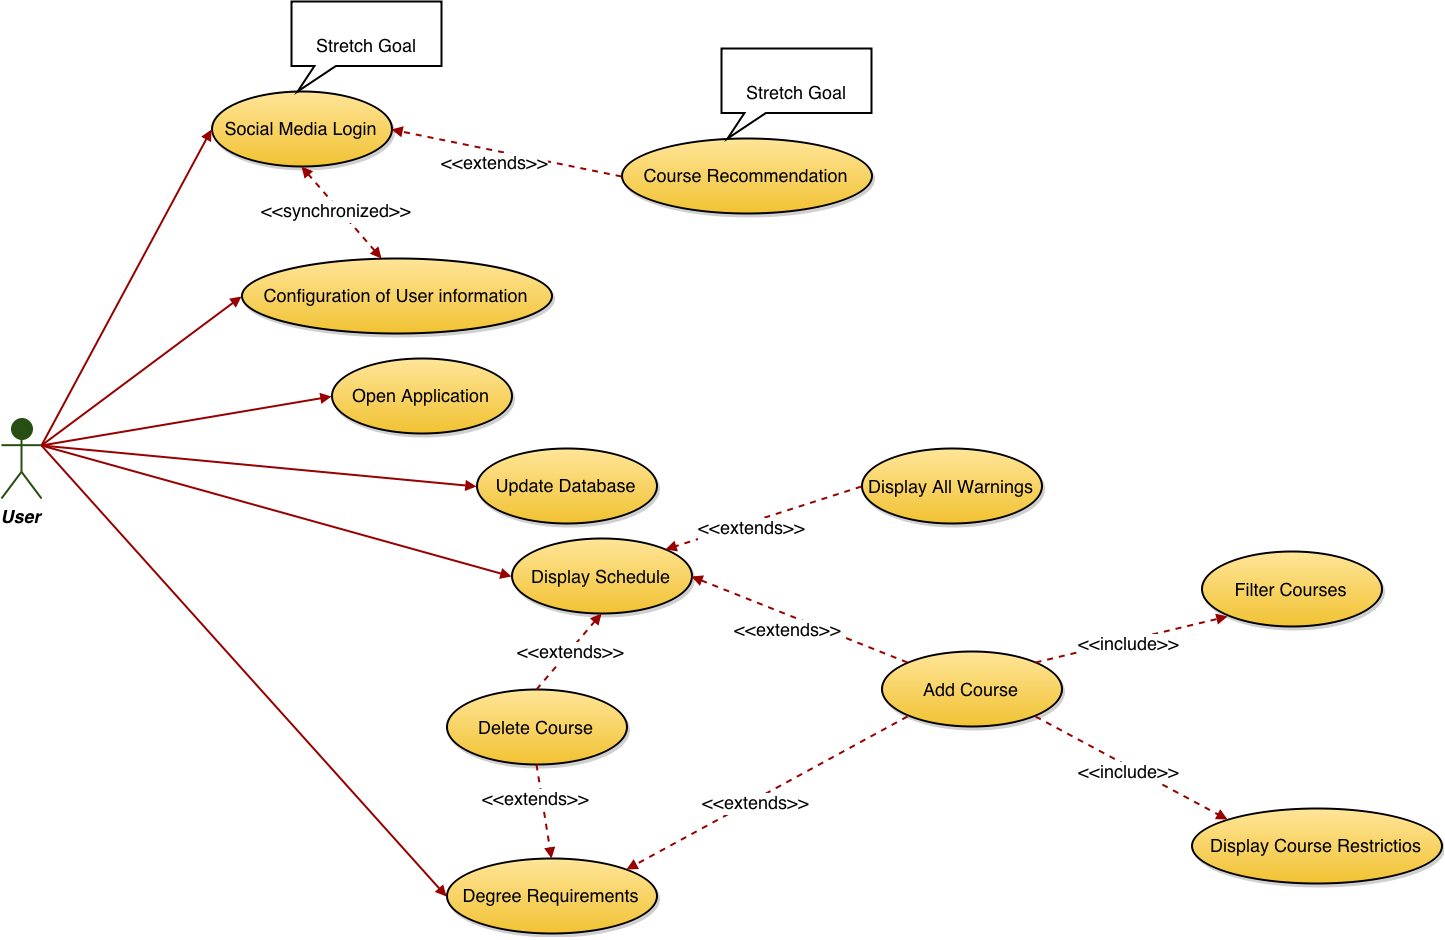
\includegraphics[width=\linewidth]{usecasediagram.png}
\caption{Use case diagram}
\label{fig:usecase_diagram}
\end{figure}

\subsection[MOCKUPS]{\selectlanguage{english}\rmfamily\bfseries\color{black}
	MOCKUPS}

{\selectlanguage{english}\color{black}
When program is opened for the first time, user encounters with configure panel. In this panel there are several different input options to configure user information (Figure \ref{fig:mockupConfig}).

\smallskip

If the user information is entered, it skips the configuration panel to the schedule panel (Figure \ref{fig:mockupSchedule}). In this panel, there is a tabbed structure for schedules. This panel has several buttons to add course, delete course and the warnings. When user clicks the buttons relevant window pops up.

\smallskip

The window for adding course to schedule has several filter options (Figure \ref{fig:mockupScheduleAdd}). In order to apply these filters to schedules the user shall click apply button, then one can see the filtered course list in the window. When they choose a course, the window is closed and returns to schedule panel.

\smallskip

To see the degree summary the user shall click menu button and the program switches the schedule panel to degree summary panel. The panel shows the summaries for all entered programs with tabbed structure. The panel also has buttons for course deletion and addition (Figure \ref{fig:mockupDegree}).}

\begin{figure}[h!]
\centering
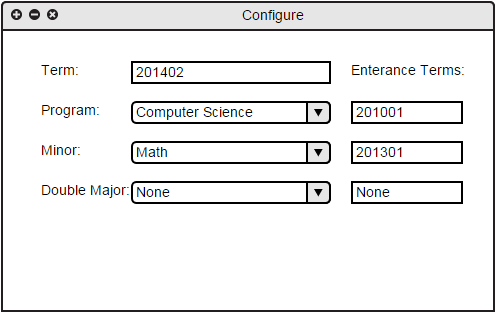
\includegraphics[keepaspectratio, scale=0.6]{Mockups/config.png}
\caption{Configuration window}
\label{fig:mockupConfig}
\end{figure}

\begin{figure}[h!]
\centering
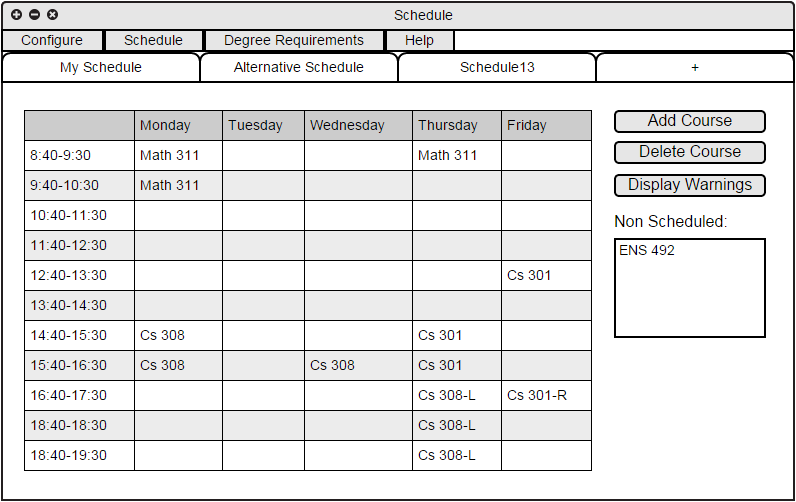
\includegraphics[keepaspectratio, scale=0.6]{Mockups/schedule.png}
\caption{Schedule panel}
\label{fig:mockupSchedule}
\end{figure}

\begin{figure}[h!]
\centering
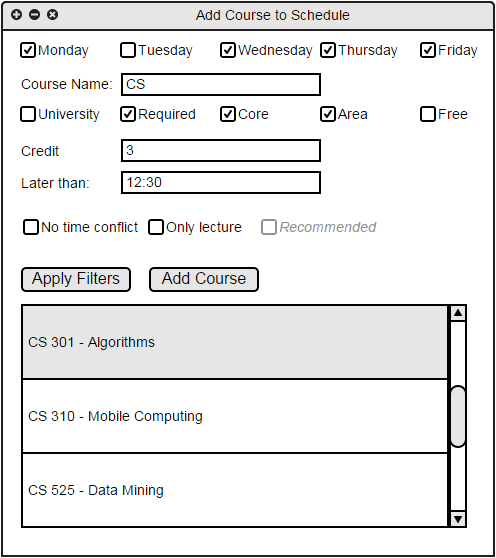
\includegraphics[keepaspectratio, scale=0.45]{Mockups/addCourseSchedule.png}
\caption{Add course window for schedule}
\label{fig:mockupScheduleAdd}
\end{figure}

\begin{figure}[h!]
\centering
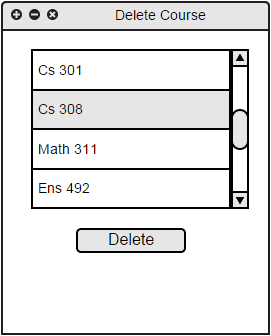
\includegraphics[keepaspectratio, scale=0.45]{Mockups/deleteCourse.png}
\caption{Delete course window}
\label{fig:mockupDelete}
\end{figure}

\begin{figure}[h!]
\centering
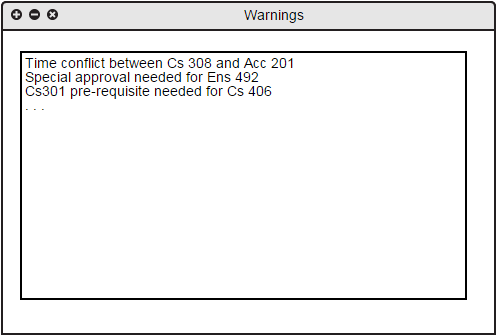
\includegraphics[keepaspectratio, scale=0.45]{Mockups/warning.png}
\caption{Warnings window for time confilct and restrictions}
\label{fig:mockupWarning}
\end{figure}

\begin{figure}[h!]
\centering
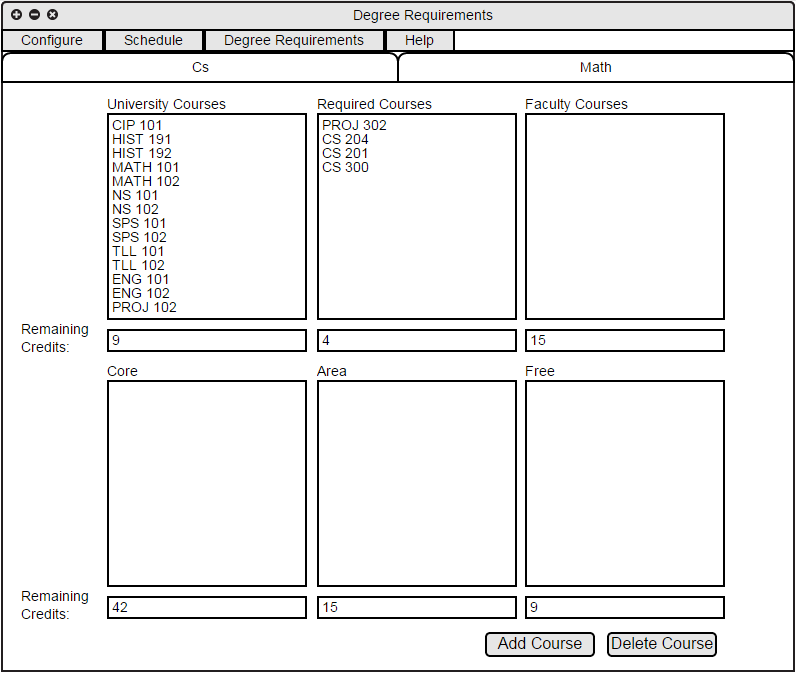
\includegraphics[keepaspectratio, scale=0.65]{Mockups/degree.png}
\caption{Panel for degree summary}
\label{fig:mockupDegree}
\end{figure}

\begin{figure}[h!]
\centering
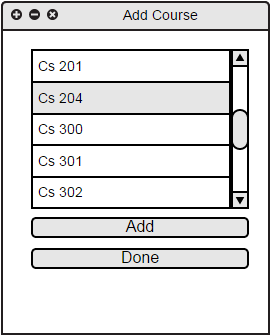
\includegraphics[keepaspectratio, scale=0.6]{Mockups/addCourseDegree.png}
\caption{Course adding window for degree summary}
\label{fig:mockupAddDegree}
\end{figure}

\clearpage\section[SYSTEM ARCHITECTURE]{\selectlanguage{english}\rmfamily\bfseries\color{black}
SYSTEM ARCHITECTURE}

{\selectlanguage{english}\color{black}
The application consists of three main components which are user interface, middleware and database. \ The main structure is shown in Figure \ref{fig:architecture_diagram} and described below.}

\begin{figure}[h]
\centering
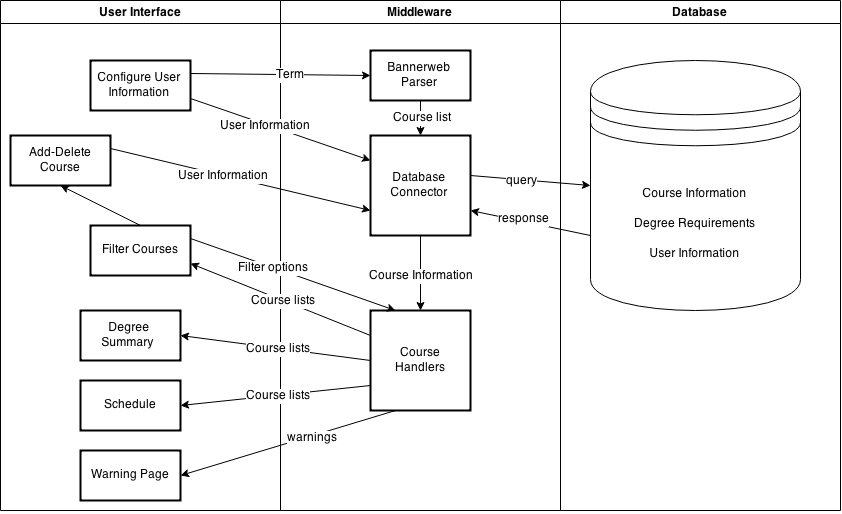
\includegraphics[width=\linewidth]{architecturediagram.png}
\caption{Architecture diagram}
\label{fig:architecture_diagram}
\end{figure}

\subsection[USER INTERFACE]{\selectlanguage{english}\rmfamily\bfseries\color{black}
USER INTERFACE}

\subsubsection[Configure user information]{\selectlanguage{english}\rmfamily\bfseries\color{black}
Configure user information}
{\selectlanguage{english}\color{black}
{Users shall enter their terms, degree program and entrance year. \ If they have minor or double major degree, it should be entered as well. \ When the user enter the information, the module passes the information to the database connector and sends the current term to bannerweb parser in order to get course list.}}

\subsubsection[Degree summary]{\selectlanguage{english}\rmfamily\bfseries\color{black}
Degree summary}
{\selectlanguage{english}\color{black}
{Users can see their completed courses and types of these courses. \ Ones can also see remaining courses to graduate in this module. \ The module will get the information from course handlers.}}

\subsubsection[Schedule]{\selectlanguage{english}\rmfamily\bfseries\color{black}
Schedule}
{\selectlanguage{english}\color{black}
{Users shall see their schedule from the graphical table which contains currently taken courses. \ The module will get the information from course handlers.}}

\subsubsection[Add delete courses]{\selectlanguage{english}\rmfamily\bfseries\color{black}
Add delete courses}
{\selectlanguage{english}\color{black}
{Users can add or delete courses to shape schedule and degree summary. \ In order to provide ease of access, this module shall cooperate with the filter courses module.}}

\subsubsection[Filter courses]{\selectlanguage{english}\rmfamily\bfseries\color{black}
Filter courses}
{\selectlanguage{english}\color{black}
{Users can filter the course list to pick with using some filter options. \ Filter module sends the filter options to middleware and gets the filtered course list from course handler. }}

\subsubsection[Warning page]{\selectlanguage{english}\rmfamily\bfseries\color{black}
Warning page}
{\selectlanguage{english}\color{black}
{This module gets the warnings from course handlers and shows to users. }}

\subsection[MIDDLEWARE]{\selectlanguage{english}\rmfamily\bfseries\color{black}
MIDDLEWARE}
\subsubsection[Database connector]{\selectlanguage{english}\rmfamily\bfseries\color{black}
Database connector}
{\selectlanguage{english}\color{black}
{Database connector generates queries to get information from database.}}

\subsubsection[Bannerweb parser]{\selectlanguage{english}\rmfamily\bfseries\color{black}
Bannerweb parser}
{\selectlanguage{english}\color{black}
{Bannerweb parser gets the specific information of courses with given term and passes to database connector.}}

\subsubsection[Course handlers]{\selectlanguage{english}\rmfamily\bfseries\color{black}
Course handlers}
{\selectlanguage{english}\color{black}
{Course handlers gets the course information and convert to specific types that user interface modules can understand.}}

\subsection[DATABASE]{\selectlanguage{english}\rmfamily\bfseries\color{black}
DATABASE}
{\selectlanguage{english}\color{black}
{The module stores the course information, degree requirement and user information with given queries.}}



\clearpage\section[SYSTEM REQUIREMENTS SPECIFICATION]{\selectlanguage{english}\rmfamily\bfseries\color{black}
SYSTEM REQUIREMENTS SPECIFICATION}


\subsection[EXTERNAL INTERFACE
REQUIREMENTS]{\selectlanguage{english}\rmfamily\bfseries\color{black}
EXTERNAL INTERFACE REQUIREMENTS}

\subsubsection[Hardware
interfaces]{\selectlanguage{english}\rmfamily\bfseries\color{black}
Hardware interfaces}
{\selectlanguage{english}\color{black}
\foreignlanguage{english}{\ }\foreignlanguage{english}{Hardware interface is a simple computer that has a network adapter. \ Since the application communicate with bannerweb, there shall be a proper internet connection.}}

\subsubsection[Software
interfaces]{\selectlanguage{english}\rmfamily\bfseries\color{black}
Software interfaces}
{\selectlanguage{english}\color{black}
\foreignlanguage{english}{\ }\foreignlanguage{english}{Since the application is a Java project, it will be a cross platform application. \ The application will be run in any operating system that has Java.}}

\subsubsection[User
interfaces]{\selectlanguage{english}\rmfamily\bfseries\color{black}
User interfaces}
{\selectlanguage{english}\color{black}
\foreignlanguage{english}{\ }\foreignlanguage{english}{The application has a graphical user interface that lets users communicate with the application via a form based window.}

\subsubsection[Other communication
interfaces]{\selectlanguage{english}\rmfamily\bfseries\color{black}
Other communication interfaces}
{\selectlanguage{english}\color{black}
\foreignlanguage{english}{\ }\foreignlanguage{english}{There will be no other communication interfaces.}}

\subsection[SYSTEM
FEATURES]{\selectlanguage{english}\rmfamily\bfseries\color{black}
SYSTEM FEATURES}


\featuresection{Time conflict handler}
\label{sssec:timeHandler}

\emph{\textbf{Input:}}  Current course and a course list that occured by the chosen courses for the current term.

\emph{\textbf{Source:}} Database that has the course information.

\emph{\textbf{Outputs:}} Boolean

\emph{\textbf{Destination:}} Main module

\emph{\textbf{Action:}} Gets the hours of the course and compares with the courses that in the list. \ It returns the value if two courses overlaping in schedule or not.

\emph{\textbf{Require:}} Non empty course list.

\emph{\textbf{Pre-condition: }} Course information is available.

\emph{\textbf{Post-condition: }} None

\emph{\textbf{Side effects:}} None



\featuresection{Time conflict filter}
\label{sssec:timeFilter}

\emph{\textbf{Input:}}  A course list that stores choosen courses and a course list to be filtered

\emph{\textbf{Source:}} Database that has the course information

\emph{\textbf{Outputs:}} Filtered course list

\emph{\textbf{Destination:}} Main module

\emph{\textbf{Action:}} Finds the courses that has no time conflict with choosen courses .

\emph{\textbf{Require:}} Time Conflict Handler

\emph{\textbf{Pre-condition: }} Course information is available.

\emph{\textbf{Post-condition: }} None

\emph{\textbf{Side effects:}} None



\featuresection{Importing course list}
\label{sssec:importCourse}

\emph{\textbf{Input:}}  Term code

\emph{\textbf{Source:}} bannerweb

\emph{\textbf{Outputs:}} None

\emph{\textbf{Destination:}} Database

\emph{\textbf{Action:}} Connects to the website with using term code, then parse the website and write the information of courses to the database.  

\emph{\textbf{Require:}} None

\emph{\textbf{Pre-condition: }} The connection to the website

\emph{\textbf{Post-condition: }} Database is updated

\emph{\textbf{Side effects:}} None



\featuresection{Importing restrictions}
\label{sssec:importRestrictions}

\emph{\textbf{Description:}} Imports the restrictions of the given course from bannerweb.

\emph{\textbf{Input:}}  Term code and CRN code

\emph{\textbf{Source:}} bannerweb

\emph{\textbf{Outputs:}} None

\emph{\textbf{Destination:}} Database

\emph{\textbf{Action:}} Connects to the website with using term code and CRN code, then parse the website and write the restrictions to the database.  

\emph{\textbf{Require:}}

\emph{\textbf{Pre-condition: }} The connection to the website

\emph{\textbf{Post-condition: }} Database is updated

\emph{\textbf{Side effects:}} None



\featuresection{Importing degree requirements}
\label{sssec:importDegree}

\emph{\textbf{Description:}} Gets degree requirements for a given degree program from bannerweb

\emph{\textbf{Input:}}  Program, Enterance year and graduation level

\emph{\textbf{Source:}} website of the given program

\emph{\textbf{Outputs:}} None

\emph{\textbf{Destination:}} Database

\emph{\textbf{Action:}} Connects to the website with using enterance year, program and graduation level, then parse the website and write the degree requirements to the database.  

\emph{\textbf{Require:}}

\emph{\textbf{Pre-condition: }} The connection to the website

\emph{\textbf{Post-condition: }} Database is updated

\emph{\textbf{Side effects:}} None

\clearpage
\subsection[SEQUENCE DIAGRAMS]{\selectlanguage{english}\rmfamily\bfseries\color{black}
SEQUENCE DIAGRAMS}

\begin{figure}[h!]
\centering
\begin{tikzpicture}
\begin{umlseqdiag} 
\umlactor[class=User]{user} 
\umlobject[class=Application, y=0.8]{app}
\umldatabase[class=Database, x=9]{db}
\begin{umlcall}[op={openApplication()}]{user}{app} 
\begin{umlfragment}[type=if, label=exist, inner xsep=5] 
\begin{umlcall}[op={isUserInformationExist()}, return={yes}]{app}{db} 
\end{umlcall}
\begin{umlcall}[op={displaySchedulePage()}]{app}{user} 
\end{umlcall}
\umlfpart[else] 
\begin{umlcall}[op={isUserInformationExist()}, return={no}]{app}{db} 
\end{umlcall}
\begin{umlcall}[op={displayConfigurePage()}]{app}{user} 
\end{umlcall} 
\end{umlfragment}
\end{umlcall}
\end{umlseqdiag} 
\end{tikzpicture}
\caption{Opening application}
\label{fig:openAppDiagram}
\end{figure}

\begin{figure}[h!]
\centering
\begin{tikzpicture}
\begin{umlseqdiag} 
\umlactor[class=User]{user} 
\umlobject[class=Application, y=0.8]{app}
\umldatabase[class=Database, x=9]{db}
\begin{umlcall}[op={openConfigurePage()},return={pageConfigure}, padding=5]{user}{app}
\end{umlcall}
\begin{umlcall}[op={formEntered()}, dt=5, padding=3]{user}{app}
\begin{umlfragment}[type=if, label={term filled}, inner xsep=11] 
\begin{umlcall}[op={getCourseList(term)}, return=courseList, dt=0]{app}{app}
\end{umlcall}
\begin{umlcall}[op={save(courseList)}, dt=4]{app}{db} 
\end{umlcall}
\end{umlfragment}
\begin{umlfragment}[type=loop, label={filled programs}, inner xsep=11 ] 
\begin{umlcall}[op={getRequirements(program)},return=requirements, dt=2]{app}{app}
\end{umlcall}
\begin{umlcall}[op={save(requirements)}, dt=4]{app}{db} 
\end{umlcall}
\end{umlfragment}
\end{umlcall}
\end{umlseqdiag} 
\end{tikzpicture}
\caption{Configure user information}
\label{fig:ConfigureDiagram}
\end{figure}

\begin{figure}[h!]
\centering
\begin{tikzpicture}
\begin{umlseqdiag} 
\umlactor[class=User]{user} 
\umlobject[class=Application, y=0.8, x=6]{app}
\begin{umlcall}[op={createNewSchedule()}]{user}{app}
\end{umlcall}
\begin{umlcall}[op={getScheduleName()}, padding=3, return=scheduleName]{app}{user}
\end{umlcall}
\begin{umlfragment}[type=while, label={scheduleName exists}, inner xsep=14] 
\begin{umlcall}[op={getScheduleName()}, padding=3, return=scheduleName, dt=6]{app}{user}
\end{umlcall}
\end{umlfragment}
\begin{umlcall}[op={displaySchedulePage(scheduleName)}, dt=6]{app}{user} 
\end{umlcall}
\end{umlseqdiag} 
\end{tikzpicture}
\caption{Create new schedule}
\label{fig:NewScheduleDiagram}
\end{figure}

\begin{figure}[h!]
\centering
\begin{tikzpicture}
\begin{umlseqdiag} 
\umlactor[class=User]{user} 
\umlobject[class=Application, y=0.8, x=6]{app}
\umldatabase[class=Database, x=12]{db}
\begin{umlcall}[op={buttonAddCourse()}]{user}{app}
\begin{umlcall}[op={getCurrentTerm()}, return={term}]{app}{db}
\end{umlcall}
\begin{umlcall}[op={getCourseList(term)}, return={courseList}]{app}{db}
\end{umlcall}
\begin{umlcall}[op={displayAddCoursePage(courseList)}]{app}{user}
\end{umlcall}
\end{umlcall}
\begin{umlcall}[op={addCourse(CRN)}, dt=4]{user}{app}
\end{umlcall}
\begin{umlcall}[op={getRestrictions(CRN)}, return={restrictions}]{app}{db} 
\end{umlcall}
\begin{umlfragment}[type=if, label={restrictions exist}]
\begin{umlcall}[op={handleRestrictions(CRN)}, return=warnings, dt=4]{app}{app}
\end{umlcall}
\begin{umlcall}[op={display(warnings)}]{app}{user}
\end{umlcall}
\begin{umlfragment}[type=case, label={confirm}, inner xsep=8]
\begin{umlcall}[op={confirm(CRN)}, dt=6]{user}{app}
\begin{umlcall}[op={save(course, scheduleName)}]{app}{db}
\end{umlcall} 
\begin{umlcall}[op={display(Done)}]{app}{user} 
\end{umlcall}
\end{umlcall}
\umlfpart[abort]
\begin{umlcall}[op={abort(CRN)}, dt=4]{user}{app}
\begin{umlcall}[op={display(Aborted)}]{app}{user} 
\end{umlcall}
\end{umlcall}
\end{umlfragment}
\umlfpart[else]
\begin{umlcall}[op={save(course, scheduleName)}]{app}{db}
\end{umlcall} 
\begin{umlcall}[op={display(Done)}]{app}{user} 
\end{umlcall}
\end{umlfragment}
\end{umlseqdiag} 
\end{tikzpicture}
\caption{Add course to schedule}
\label{fig:AddCourseScheduleDiagram}
\end{figure}

\begin{figure}[h!]
\centering
\begin{tikzpicture}
\begin{umlseqdiag} 
\umlactor[class=User]{user} 
\umlobject[class=Application, y=0.8, x=6]{app}
\begin{umlcall}[op={buttonFilterCourse()}]{user}{app}
\begin{umlcall}[op={PageFilterCourse(courseList)}, return=filters]{app}{user}
\end{umlcall}
\end{umlcall}
\begin{umlcall}[op={filter(courseList,filters)}, return=courseList]{app}{app}
\end{umlcall}
\begin{umlcall}[op={updatePageAddCourse(courseList)}]{app}{user}
\end{umlcall}
\end{umlseqdiag} 
\end{tikzpicture}
\caption{Filter course list for schedule}
\label{fig:FilterCourseScheduleDiagram}
\end{figure}

\begin{figure}[h!]
\centering
\begin{tikzpicture}
\begin{umlseqdiag} 
\umlactor[class=User]{user} 
\umlobject[class=Application, y=0.8]{app}
\umldatabase[class=Database, x=9]{db}
\begin{umlcall}[op={buttonDeleteCourse()}]{user}{app}
\begin{umlcall}[op={getCourse()}, return=CRN]{app}{user}
\end{umlcall}
\begin{umlcall}[op={delete(CRN, scheduleName)}]{app}{db}
\end{umlcall}
\begin{umlcall}[op={display(Done)}]{app}{user}
\end{umlcall}
\end{umlcall}
\end{umlseqdiag} 
\end{tikzpicture}
\caption{Delete course from schedule}
\label{fig:UpdateDiagram}
\end{figure}

\begin{figure}[h!]
\centering
\begin{tikzpicture}
\begin{umlseqdiag} 
\umlactor[class=User]{user} 
\umlobject[class=Application, y=0.8]{app}
\umldatabase[class=Database, x=11]{db}
\begin{umlcall}[op={buttonUpdate()}]{user}{app}
\begin{umlcall}[op={getCurrentTerm()}, return=term]{app}{db}
\end{umlcall}
\begin{umlcall}[op={getCoursesFromBanneweb(term)}]{app}{app}
\begin{umlcall}[op={deleteCourseList(term)}, dt=4]{app}{db}
\end{umlcall}
\begin{umlcall}[op={save(courseList, term)}]{app}{db}
\end{umlcall}
\begin{umlcall}[op={display(Done)}]{app}{user}
\end{umlcall}
\end{umlcall}
\end{umlcall}
\end{umlseqdiag} 
\end{tikzpicture}
\caption{Update database}
\end{figure}

\begin{figure}[h!]
\centering
\begin{tikzpicture}
\begin{umlseqdiag} 
\umlactor[class=User]{user} 
\umlobject[class=Application, y=0.8, x=5]{app}
\umldatabase[class=Database, x=10]{db}
\begin{umlcall}[op={buttonAddCourse()}]{user}{app}
\begin{umlcall}[op={getCourseListForDegree()}, return=courseList]{app}{db}
\end{umlcall}
\begin{umlcall}[op={PageAddCourse(courseList)}, return=courseName]{app}{user}
\end{umlcall}
\begin{umlcall}[op={addTakenCourse(courseName)}]{app}{db}
\end{umlcall}
\begin{umlcall}[op={display(Done)}]{app}{user}
\end{umlcall}
\end{umlcall}
\end{umlseqdiag} 
\end{tikzpicture}
\caption{Add course to degree requirements}
\label{fig:addDegree}
\end{figure}

\begin{figure}[h!]
\centering
\begin{tikzpicture}
\begin{umlseqdiag} 
\umlactor[class=User]{user} 
\umlobject[class=Application, y=0.8, x=6]{app}
\umldatabase[class=Database, x=12]{db}
\begin{umlcall}[op={buttonAddCourse()}]{user}{app}
\begin{umlcall}[op={getCourseListForDegree()}, return=courseList]{app}{db}
\end{umlcall}
\begin{umlcall}[op={PageAddCourse(courseList)}, return=courseName]{app}{user}
\begin{umlcall}[op={onChangedFilterBox()},]{user}{app}
\begin{umlcall}[op={filter(courseList,filterText)}, return=courseList]{app}{app}
\end{umlcall}
\begin{umlcall}[op={updatePageAddCourse(courseList)}]{app}{user}
\end{umlcall}
\end{umlcall}
\end{umlcall}
\begin{umlcall}[op={addTakenCourse(courseName)}]{app}{db}
\end{umlcall}
\begin{umlcall}[op={display(Done)}]{app}{user}
\end{umlcall}
\end{umlcall}
\end{umlseqdiag} 
\end{tikzpicture}
\caption{Add course to degree requirements with filter}
\label{fig:filterDegree}
\end{figure}

\begin{figure}[h!]
\centering
\begin{tikzpicture}
\begin{umlseqdiag} 
\umlactor[class=User]{user} 
\umlobject[class=Application, y=0.8, x=5]{app}
\umldatabase[class=Database, x=11]{db}
\begin{umlcall}[op={buttonDeleteCourse()}]{user}{app}
\begin{umlcall}[op={getCourse()}, return=courseName]{app}{user}
\end{umlcall}
\begin{umlcall}[op={deleteTakenCourse(courseName)}]{app}{db}
\end{umlcall}
\begin{umlcall}[op={display(Done)}]{app}{user}
\end{umlcall}
\end{umlcall}
\end{umlseqdiag} 
\end{tikzpicture}
\caption{Delete course from degree requirements}
\label{fig:deleteDegree}
\end{figure}

\begin{figure}[h!]
\centering
\begin{tikzpicture}
\begin{umlseqdiag} 
\umlactor[class=User]{user} 
\umlobject[class=Application, y=0.8]{app}
\umlobject[class=Social media, y=0.8]{sm}
\umldatabase[class=Database]{db}
\begin{umlcall}[op={buttonSocialMedia()}]{user}{app}
\begin{umlcall}[op={getCredentials()}, return=credentials]{app}{user}
\end{umlcall}
\begin{umlcall}[op={validate(credentials)}, return=boolean]{app}{sm}
\end{umlcall}
\begin{umlfragment}[type=while, label={valid credentials}, inner xsep=14] 
\begin{umlcall}[op={getCredentials()}, return=credentials]{app}{user}
\end{umlcall}
\begin{umlcall}[op={validate(credentials)}, return=boolean]{app}{sm}
\end{umlcall}
\end{umlfragment}
\begin{umlfragment}[type=if, label={logged in before}, inner xsep=14] 
\begin{umlcall}[op={getUserInfo()}, return=userInfo, dt=4]{app}{sm}
\end{umlcall}
\begin{umlcall}[op={update(userInfo)}, dt=4]{app}{db} 
\end{umlcall}
\umlfpart[else]
\begin{umlcall}[op={getUserInfo()}, return=userInfo, dt=4]{app}{db}
\end{umlcall}
\begin{umlcall}[op={update(userInfo)}, dt=4]{app}{sm} 
\end{umlcall}
\end{umlfragment}
\end{umlcall}
\end{umlseqdiag} 
\end{tikzpicture}
\caption{Social media login}
\label{fig:SocialMediaDiagram}
\end{figure}

\begin{figure}[h!]
\centering
\begin{tikzpicture}
\begin{umlseqdiag} 
\umlactor[class=User]{user} 
\umlobject[class=Application, y=0.8, x=5]{app}
\umlobject[class=Social media, y=0.8, x=9]{sm}
\umldatabase[class=Database]{db}
\begin{umlcall}[op={buttonRecommendation()}]{user}{app}
\begin{umlcall}[op={isLoggedIn()}]{app}{sm} 
\end{umlcall}
\begin{umlfragment}[type=if, label={logged in}, inner xsep=9] 
\begin{umlcall}[op={getRecommendation()}, return=courseList, dt=4]{app}{sm}
\begin{umlcall}[op={generateRecommendation()}, return=courseList, dt=4]{sm}{sm}
\end{umlcall}
\end{umlcall}
\begin{umlcall}[op={getTimeAndSchedule(courseList)}, return=courseList, dt=4]{app}{db} 
\end{umlcall}
\begin{umlcall}[op={display(courseList)}, dt=4]{app}{user}
\end{umlcall}
\umlfpart[else]
\begin{umlcall}[op={display(notLoggedIn)}, dt=4]{app}{user}
\end{umlcall}
\end{umlfragment}
\end{umlcall}
\end{umlseqdiag} 
\end{tikzpicture}
\caption{Course recommendation}
\label{fig:RecommendationDiagram}
\end{figure}


\end{document}
